\section{Unfolding the matrix power} 
\label{sec:appendix-unfold}
In this appendix, we define formally the unfolding function described in Section~\ref{sec:unfolding}, by induction on the size of the input term. For the inductive step, we will call the unfolding function on a very specific class of terms called \emph{shallow terms} and defined below. We define unfolding for these shallow terms and generalize it, via induction, to the whole class to terms.

\subsection{Shallow terms and their unfolding}\label{sec:shallow-terms}

\paragraph*{Shallow terms.} Let us describe the shallow-terms datatype. For now, it is just an intermediary type to define formally the unfolding function. Later on, we will use it as a basic datatype when we will decompose the unfolding function into smaller prime functions (see Appendix~\ref{ap:matrix-power}). 

 Let $\rSigma$ and $\rGamma$ be two ranked sets. An element of the shallow terms datatype denoted $\shallowterm \rSigma \rGamma$, is an expression of the form $a\tensorpair{b_1,\dots,b_n}$ where $a$ is an $n$-ary element of $\rSigma$ and $b_1,\dots, b_n$ are elements of $\rGamma$. We draw shallow terms like this:
\mypic{54}
Clearly, a shallow term is just a particular case of terms.


Unfolding of shallow terms is the function of type 
\begin{align*}
    \ranked{
        \xymatrix{
            \shallowterm{\mati k \rSigma} {\mati k \rGamma}  \ar[r] & \mati k {(\shallowterm \Sigma \Gamma)}.
        }
    }
\end{align*}
which is the restriction of the more general unfolding function we want to define to shallow terms. Here is a picture of unfolding for shallow terms:
\begin{center}
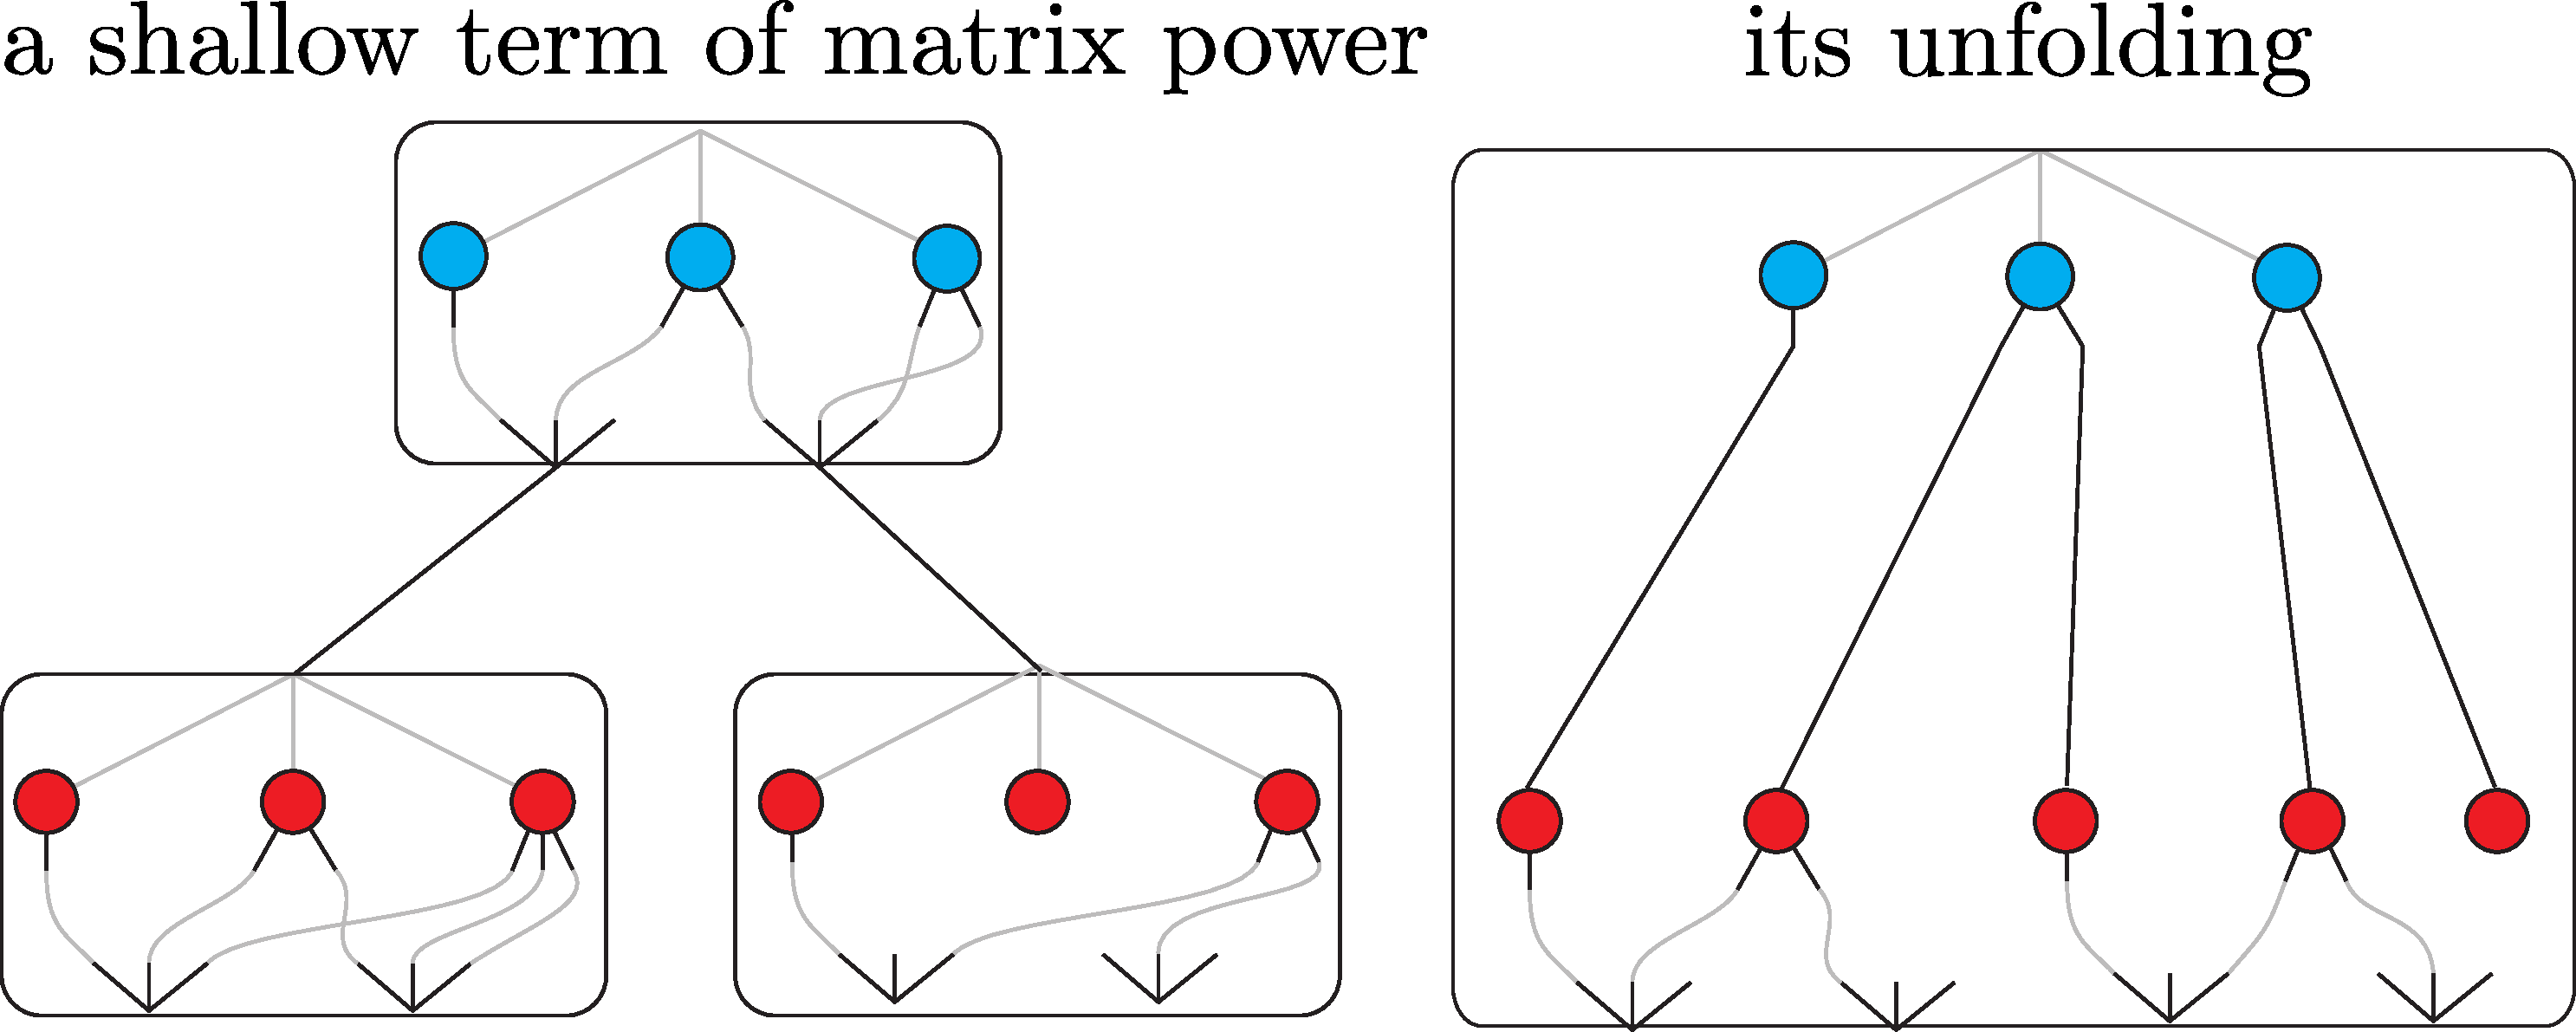
\includegraphics[scale=.17]{pictures/shallow-term-unfold}
\end{center}
To define it formally, we will introduce three functions manipulating shallow terms. Here again, these functions, which are used here as an intermediary functions to define the unfolding formally, will become prime functions when we will decompose the unfolding function.

\paragraph*{Functions on shallow terms.} Let $\rGamma$ and $\rSigma$ be two datatypes.  Consider the function $f$
\begin{align*}
\ranked{\shallowterm  \Gamma {\reduce k \Sigma} \xrightarrow{\quad f\quad} \reduce k(\shallowterm  \Gamma  \Sigma)} 
\end{align*}
illustrated by the following picture  
\begin{center}
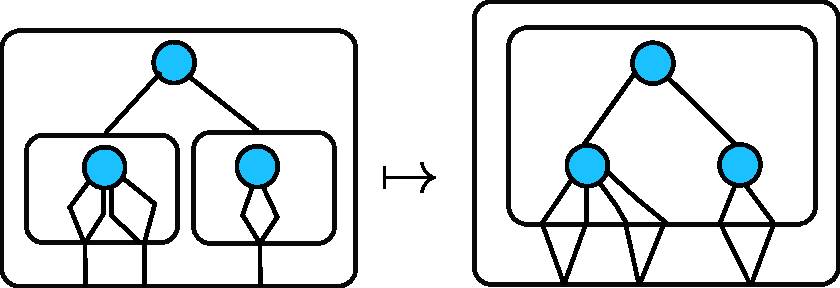
\includegraphics[scale=.4]{pictures/shallow-fold-distrib}
\end{center}
and defined as follows. 

Let $g$ be the function of type
\begin{align*}
\ranked{\shallowterm  {\reduce k \Gamma} {\Sigma^k} \xrightarrow{\quad g\quad} \reduce 1 (\shallowterm  \Gamma  \Sigma)} 
\end{align*}
illustrated by the following picture  
\begin{center}
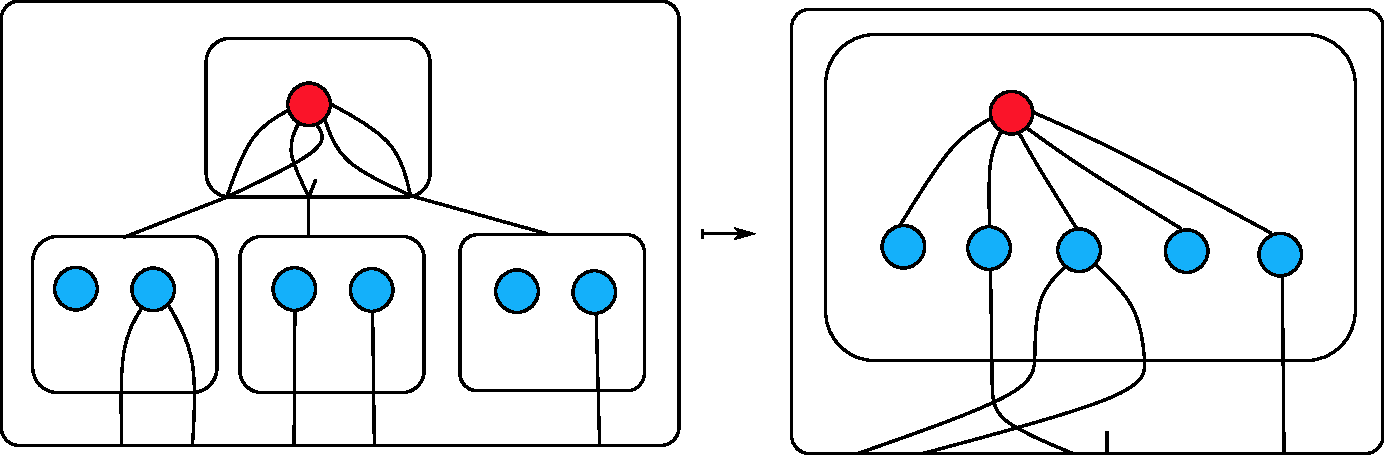
\includegraphics[scale=.37]{pictures/shallow-unfold}
\end{center}
and defined as follows. 

Finally consider the function $h$
\begin{align*}
\ranked{\shallowterm  {\Gamma^k} {\Sigma} \xrightarrow{\quad h\quad} (\shallowterm  \Gamma  \Sigma)^k} 
\end{align*}
illustrated by the following picture  
\begin{center}
{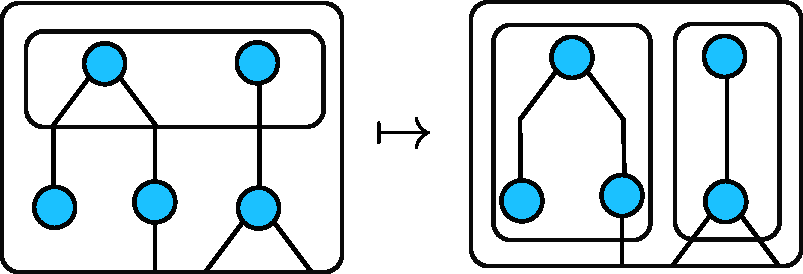
\includegraphics[scale=.4]{pictures/tensor-shallow-distrib}}
\end{center}
and defined as follows. 

\paragraph*{Unfolding shallow terms.} Unfolding for shallow terms is defined to be  the composition of the following functions
  \begin{align*}
  \xymatrix@C=2.8cm{
          \ranked{\shallowterm{\mati k \rSigma} {\mati k \rGamma} = {\shallowterm{\reduce k {\Sigma^k}}{\reduce k {\Gamma^k}}} 
        \ar[d]_{\ranked{\substack{f}}}
        \ar[r]^-{\ranked{\text{Shallow unfold}}}}
        &
        \ranked{ \reduce k(\shallowterm{\Sigma}{ {\Gamma}})^k = \mati k {(\shallowterm \Sigma \Gamma)}}
        \\
       \ranked{  \reduce k(\shallowterm{\reduce k {\Sigma^k}}{ {\Gamma^k}})}
        \ar[r]_-{\ranked{\flatt\circ \reduce k g}}
        &
    \ranked{   \reduce k(\shallowterm{\Sigma^k}{ {\Gamma}}) } \ar[u]^{\ranked{\reduce k  h}}
    } 
\end{align*}    

\subsection{Definition of unfolding}
Let us define now define the unfolding function for arbitrary inputs.
Unfolding is the function of type 
\begin{align*}
    \ranked{\unfold : \tmonad \mati k \rSigma \to \mati k {(\tmonad \Sigma)} }
    \end{align*}
    which  is defined as follows by induction on the size of the input term. If the input is an empty term, then the output is this term:
\mypic{83}
Otherwise, if the input is a nonempty term $a(t_1,\ldots,t_n)$ then the output is obtained by first applying term unfolding to to the smaller terms $t_1,\ldots,t_n$, and then applying the shallow unfold. 